\section{Umsetzung}
% Fully corrected!
Im Folgenden werden die verschiedenen Ansätze zur Lösung des Problems dieser Arbeit betrachtet und dargelegt. Dabei soll besonders die verschiedenen Möglichkeiten beleuchtet werden, um somit auch Vergleiche zwischen den Technologien anstellen zu können.\\\\
Als Vorbereitung zur Implementation und dem späteren Training gilt es zunächst eine Datengrundlage zu schaffen, auf welcher der Trainingsprozess stattfinden kann. Für diese Datengrundlage gilt der Anspruch, dass sie möglichst umfassend ist und somit im gesamtem Training der KI möglichst viele diverse Situationen abbildet, um somit den Trainingserfolg in der Theorie zu maximieren.\\
Damit dieser Anspruch erfüllt werden kann, aber gleichzeitig der benötigte Aufwand für das Sammeln der Daten sowie das Auswerten dieser minimal gehalten wird, bietet sich die Verwendung eines Simulators an. In diesem simulierten Umfeld kann die KI gegen sich selbst antreten und somit anhand dieser Erfahrungen lernen. Dies bedeutet, dass ein Modell geschaffen werden muss, welches der Realität möglichst gut entspricht, um somit die Lernergebnisse der KI überhaupt in der Realität nutzbar zu machen.\\\\
Mit dem funktionierenden Simulator kann dann die Entwicklung einer KI begonnen werden, welche mit dem simulierten Umfeld interagieren kann und dieses entsprechend die benötigten Informationen zur Entscheidungsfindung bereitstellt. Mit diesen Komponenten und einem Ansatz zur korrekten Bewertung der KI Entscheidungen im Lernprozess kann ein zielführendes Training der KI erfolgen.\\\\
Die KI-Entwicklung fußt zunächst auf einer Entscheidung der korrekten Technologien und Algorithmen für das vorliegende Problem. Im Weiteren können die einzelnen Parameter anhand von Daten des Lernprozesses eines Prototypen verfeinert werden, sodass schlussendlich für jeden verfolgten Ansatz eine belegbar optimale Performance erzielt wird.\\\\
Anschließend zur Entwicklung werden die verschiedenen Ansätze bewertet und gegenseitig in Kontext gesetzt, um somit abschließend einen möglichst geeigneten Prototypen vorstellen zu können.

\subsection{Technologie Entscheidung}
%Fully Corrected
Durch den Umstand, dass die bevorstehenden Aufgaben maßgeblich mit dem Umgang von Daten und der Implementation einer KI geprägt sind, wird zur Umsetzung im Folgenden hauptsächlich auf die Programmiersprache \gqq{Python} gesetzt. Diese zeichnet sich besonders bei der Implementation von künstlichen Intelligenzen durch bestehende und umfangreiche Bibliotheken aus. Zusätzlich ist die Kompetenz im Team der Autoren im Umgang mit Python sehr hoch und erleichtert somit den Einstieg in die künstliche Intelligenz.\\\\
%TODO umformulieren und ausbauen
Mit Blick auf die ausgewählte Programmiersprache stehen zur Umsetzung der KI verschiedene Bibliotheken zur Verfügung, die bereits Strukturen zur Implementierung neuronaler Netze bereitstellen.\\
Zweck eines solchen Frameworks ist es, die Entwicklung der Algorithmen des maschinellen Lernens zu Vereinfachen und dem Nutzer einen gewissen Grad an Abstraktion zu bieten, sodass er sich im Wesentlichen nicht um die zugrunde liegenden mathematischen Prinzipien entsprechend den Ausführungen in \ref{künstliches_neuron} und \ref{lernprozess} kümmern muss. Hierbei bieten im Allgemeinen verschiedene Bibliotheken einen unterschiedlichen Grad der Abstraktion.\\
Zur Entscheidung für ein geeignetes Frameworks werden nachfolgend die weitverbreiteten Bibliotheken Tensorflow und PyTorch betrachtet.
\begin{itemize}
    \item Tensorflow:\\\\
    Das ursprünglich als interne Lösung von Google entwickelte und seit 2015 veröffentlichte Machine-Learning-Framework Tensorflow gehört mit zu den verbreitetsten und bekannten Lösungen für die Implementierung neuronaler Netze. Als eine der wichtigsten Eigenschaften von Tensorflow gilt der Grad an Abstraktion, den der Entwickler %TODO nachdenken ob gendern
    durch die Verwendung dieser Bibliothek erreichen kann. So muss sich der Nutzende nicht mit den zugrunde liegenden Details neuronaler Netze auseinandersetzen, sondern kann sich auf die übergeordnete Logik des zu implementierenden Anwendungsfalls beziehungsweise des abzubildenden Modells konzentrieren. Weiterhin gilt Tensorflow als Framework, welches eine gute Erweiterbarkeit beziehungsweise Skalierbarkeit ermöglicht.
    Im Allgemeinen stehen Schnittstellen zur Verfügung, die die Verwendung verschiedenster Programmiersprachen im Zusammenspiel mit Tensorflow erlauben, darunter auch Python.\zitat{}{pytorchtensorflow}
    \\
    \item PyTorch:\\\\
    Die in erster Version 2018 veröffentliche Machine-Learning-Bibliothek PyTorch stellt eine Lösung mit wachsender Popularität und Verbreitung für die Realisierung neuronaler Netze dar. Sie basiert dabei zu wesentlichen Teilen auf dem mittlerweile veralteten LuaTorch, einer Bibliothek zur Durchführung wissenschaftlicher Berechnungen.\\
    PyTorch gilt als Bibliothek welche eine besonders python-typische Umsetzung neuronaler Netze ermöglicht und hierzu Interfaces bereitstellt, welche python-erfahrenen Entwicklern einen intuitiven Umgang mit dem Framework ermöglichen. Weiterhin gilt PyTorch als Framework welches sich durch seine Flexibilität auszeichnet, besonders hinsichtlich der Möglichkeiten des Debuggings und Testings.\zitat{}{pytorchtensorflow}
\end{itemize}
Mit Blick auf die vorgestellten Bibliotheken wurde sich für die Verwendung von PyTorch entschieden. Gründe hierfür sind zum einen die bereits erwähnte Kompetenz der Entwickler in der Programmiersprache Python, aus welcher sich durch die Verwendung von PyTorch eine schnelle Einarbeitung und intuitive Entwicklung ergibt. Ein weiterer positiver, wenngleich nicht entscheidungskritischer Aspekt ist die höhere Performance von PyTorch gegenüber dem Machine-Learning-Framework Tensorflow.\zitat{}{performancePytorchTensorflow}\\\\
Es ist anzumerken, dass trotz der Entscheidung für PyTorch die implementierten Algorithmen keine Funktionalitäten verwenden, die spezifisch für die gewählte Bibliothek sind. Somit lässt sich die nachfolgend dargestellte Umsetzung des neuronalen Netzes beziehungsweise der künstlichen Intelligenz grundsätzlich ohne Weiteres mithilfe von alternativen Bibliotheken und vergleichbaren Tools umsetzen.

\subsection{Rennsimulator}
% Fully Corrected
Um unsere KI trainieren zu können, bedarf es eine aussagekräftige Datengrundlage, welche umfassend diverse Situationen abbildet. Nur in diesem Fall kann die KI tatsächliche Strategien erlernen, welche als solche dann in den realen Anwendungsfall übertragen werden können. Da seit dem Jahr 2017 in der Formel 1 eine neue Art Reifen gefahren wird, welche an der Vorder- sowie Hinterachse am Fahrzeug breiter sind und zusätzlich aus moderneren Mischungen bestehen, können als reale Datengrundlage nur die Rennen von 2017 bis zum jetzigen Stand Ende 2021 benutzt werden. In diesem Zeitraum wurden die Mischungen vom Zulieferer der Reifen zwar leicht angepasst, dennoch wird hierbei aufgrund der identischen Abmessungen zu den Reifen bis Ende der Saison 2021 von einer gegebenen Vergleichbarkeit ausgegangen. Entsprechend stehen nur 100 Rennen als Datengrundlage zur Verfügung, was für das Training einer KI unzureichend ist und uns somit zwingt, eine andere Methode zu wählen, um eine aussagekräftige und möglichst diverse Umgebung zu schaffen, in welcher die KI die umfassenden Möglichkeiten eines Formel 1 Rennens kennen und verstehen lernen kann. Daher wurde im Team die Entscheidung getroffen, einen Simulator für ein Rennen zu schreiben, welcher auf Modellen und Abstraktionen beruht, die durch die Erhebung der Datenmenge über den Zeitraum von 2018 - 2021 erfolgen. Diese Modelle werden dann genutzt, um beispielsweise den Reifenverschleiß pro Runde simulieren zu können und sollen dabei das Verständnis des Zusammenhangs zwischen der Abnutzung des Reifens und der noch bestmöglichen Rundenzeit liefern. Gerade dieser Zusammenhang ist ein Kernpunkt in Bezug auf den Erfolg des Simulators, da der Traktionsverlust pro Runde durch den zunehmend verschlissenen Reifen maßgeblich die Rennstrategie und den optimalen Zeitpunkt des Boxenstopps bestimmt.

\subsubsection{Anforderungen}
% Fully corrected!!!
% Realitätsnah, Zeitlich weniger Aufwand -> Arbeit soll KI nicht Sim, Skalierbar -> weil ausgeklammert,  
Die Anforderungen gegenüber des Simulators beschränken sich im Kern auf eine möglichst genaue Abstraktion der Wirklichkeit, um somit die Relevanz und Nutzbarkeit der von uns entwickelten KI sicherzustellen und zu gewährleisten. Aufgrund des zeitlichen Rahmens dieser Arbeit wird hierbei aber die Notwendigkeit des Ausklammerns von möglichen Einflüssen genannt, um damit zu Beginn der Arbeit die Komplexität in der Entwicklung und später im Training der KI zu reduzieren und somit sich zunächst auf einen aussagekräftigen Prototypen zu beschränken. Beispielsweise könnte initial auf jegliche Abbildung von Wetter und Luft- wie Streckentemperatur verzichtetet werden und dennoch ein robuster Simulator für trockene Wetterverhältnisse geschaffen werden. Folgend dieser möglichen Notwendigkeit der Reduktion von berücksichtigen Faktoren soll bei der Entwicklung des Simulators besonders in der Architektur auf die Skalierbarkeit dieser geachtet werden, um somit die nachfolgende Erweiterung ohne umfassenden zeitlichen Aufwand zu ermöglichen.

Die in dieser Arbeit untersuchten Faktoren und somit Anforderungen an unseren Simulator sind umfassend durch den Reifenverschleiß, der individuellen Leistung eines einzelnen Fahrzeuges in Kombination mit dem Fahrer und den Wechselwirkungen der Fahrzeuge untereinander gegeben. Diese Einflüsse sollen durch das geeignete Modell im Simulator widergespiegelt und berücksichtigt werden.

\newpage %TODO may be not necessary; shall prevent fig:sim_architecture to behave random
\subsubsection{Architektur} \label{sim_architecture_header}
% Fully corrected
% Diskrete Eventsimulation, gewährleisten von Skalierbarkeit, OOP, Performance, Technologie Entscheidung Python weil Anbindung an KI Libs
\begin{figure}[H]
    \centering
    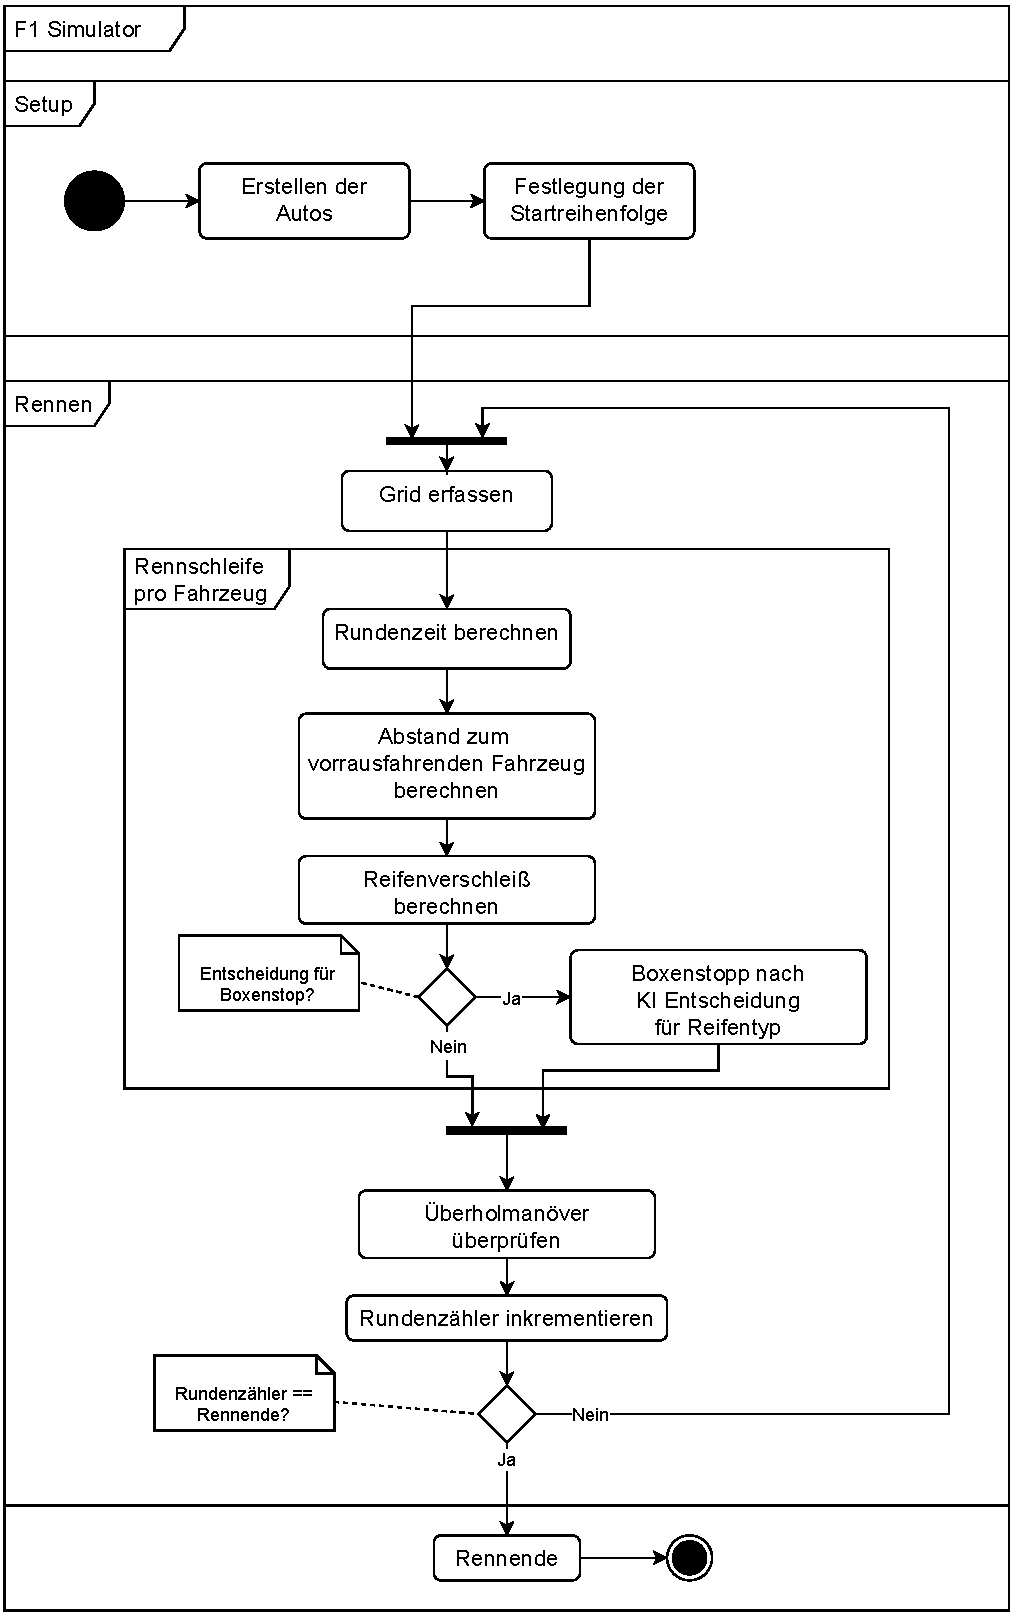
\includegraphics[scale=0.80]{Studienarbeit_F1/images/diagrams/f1_sim_architecture_overview_crop.pdf}
    \caption{Systemablaufmodell des Simulators}
    \label{fig:sim_architecture}
\end{figure}

Aus architektonischer Sicht muss besonders die angestrebte Skalierbarkeit des Simulators beachtet werden. Diese soll erlauben, zu späteren Ständen des Projektes ohne große Eingriffe und völlig ohne Umstrukturierung neue Faktoren und Funktionen in die Simulation einzubinden und somit zunehmend den Grad der Abstraktion zu reduzieren und dadurch die Aussagekraft zu erhöhen. Mit Berücksichtigung dieses Ziels wurde die grobe Architektur wie in der Abbildung \ref{fig:sim_architecture} entworfen. Dabei ist besonders die \gqq{Rennschleife} als zentraler Punkt der Architektur zu beachten, da diese so ausgelegt ist, dass jederzeit neue Funktionen eingehängt werden können und somit die Einflüsse modular erweitert werden können. Diese Architektur ist dabei an den \gqq{Single Threaded Main Event Loop} angelehnt, welcher mehrere Anfragen einzeln in einer Hauptschleife abarbeitet, dafür aber für jede eigentlich blockierende Operation einen eigenen Thread eröffnet.\cite{pattern_oriented_architecture} Den zuletzt genannten Aspekt der Generation von neuen Threads wird in unserem Ansatz nicht weiter verfolgt. Um die Modularität zusätzlich zu erreichen, werden alle Fahrzeuge sowie deren Attribute als Objekte der entsprechenden Klassen abgebildet und erlauben so den Zugriff aus jeglichen Bereichen des Systems über eine zentrale Speicheradresse der Objekte. Weiter ist die Entkopplung des Erstellens der Fahrzeuge und somit der Startaufstellung vom eigentlichen Renngeschehen zu beachten. Dies soll ermöglichen, mehrere Rennen hintereinander mit der gleichen Generation an Fahrzeugen mit gleicher Verteilung in der Startaufstellung abzubilden.

\subsubsection{Erhebung der Daten}
% Fully corrceted
% Wo kommen die Daten her und wie werden sie zielgerichtet ausgewertet? Welche Daten sind interessant?
In der Startphase des Projektes wurde auf der in \ref{sim_architecture_header} erdachten Architektur ein Prototyp erarbeitet, welcher erlaubte die Machbarkeit sowie die angestrebte Skalierbarkeit des Simulators zu prüfen. Für die Abstraktion der diversen Sachverhalte, wie beispielsweise Reifenverschleiß wurde bei dieser Grundversion aber auf die Untersuchung jeglicher Datengrundlage verzichtet, um erst einmal bei einem Prototyp zu bleiben. Nach erfolgreicher Integration einer KI in den bestehenden Prototypen wurde in der zweiten Phase des Projektes die fehlende Wissenschaftlichkeit des Simulators adressiert. Dies geschah durch die umfassende Analyse von relevanten Daten im Zielkontext, welche zunächst ausgewählt und aufbereitet wurden. Das Ziel ist hierbei: Gewährleistung der realitätsnahen Aussagekraft des Simulators zur Sicherstellung der Anwendbarkeit der resultierenden KI.
\\\\
Die nötigen Daten wurden durch die Python-Library \gqq{Fast F1} \cite{fast_f1} zur Verfügung gestellt. Diese API (Application Programming Interface) zeichnet sich besonders durch die umfangreiche Menge und einem hohen Detailgrad an Daten aus, welche historisch bis zum Jahr 2016 zurückreichen. So stehen uns jegliche Informationen auf die Runde genau von jedem einzelnen Fahrzeug zur Verfügung. Dies erlaubt somit für jeden Typen Reifen ein einzelnes und aussagekräftiges Modell zu generieren. Hierfür wurde zunächst ein Parser erstellt, welcher aus den bereitgestellten Daten die für unsere Anwendung relevanten Daten herausfiltert und diese im JSON-Format nach Rennwochenende sortiert speichert. Hierbei kann dem Parser ein beliebiges Jahr sowie eine beliebige Rennwochenende übergeben werden, deren Daten anschließend nach Reifenmischung sortiert abgelegt werden. Hierfür werden die Daten für alle drei Mischungsarten untersucht und für ein jedes Auto die verwendeten Reifen eines jeden Stints untersucht und abgespeichert. Ein Stint bezeichnet hierbei den Rennabschnitt, in welchem der Reifen gefahren wird. Heißt startet ein Fahrzeug auf der Mischung \gqq{Soft} und wechselt dann in Runde \gqq{x} auf die Mischung \gqq{Medium} so wird die Renndistanz vom Start bis Runde \gqq{x} als ein Stint bezeichnet. Anschließend können damit für jeden verwendeten Reifen die Nutzungsdauer sowie die während dieser Nutzung geleisteten Rundenzeiten analysiert werden, um die Relation zwischen möglicher Rundenzeit und dem Verschleiß des Reifens zu untersuchen. Hierbei kann bei Bedarf auch der einzelne Fahrer spezifiziert werden, um die eben beschriebene Auswertung nur im Kontext eines Fahrers zu betreiben, und somit die Varianz der diversen Fahrer und Fahrzeuge ausschließen zu können.\\
Zusätzlich bietet die \gqq{Fast F1} API bereits die Option, die Daten nach Relevanz vorzufiltern. Dies bedeutet im Kontext der Formel 1, dass alle Rundenzeiten, welche nicht aussagekräftig für die Leistung des Fahrzeuges sind, bereits ausgeklammert werden. Eine Runde in der Formel 1 verliert aus Daten-technischer Sicht dann an Bedeutung, wenn in dieser Runde kein normales Renntempo gehalten werden konnte. Dies geschieht beispielsweise im Falle eines Unfalls auf der Strecke und den zugehörigen gelben Flaggen beziehungsweise dem Einsatz des \gqq{Safety Cars} oder einem vollständigem Rennabbruch bei roter Flagge.
% Bild von quick_plotter.py als Beispiels für die eben eingeführten und erklären Konzepte!
\begin{figure}[H]
    \centering
    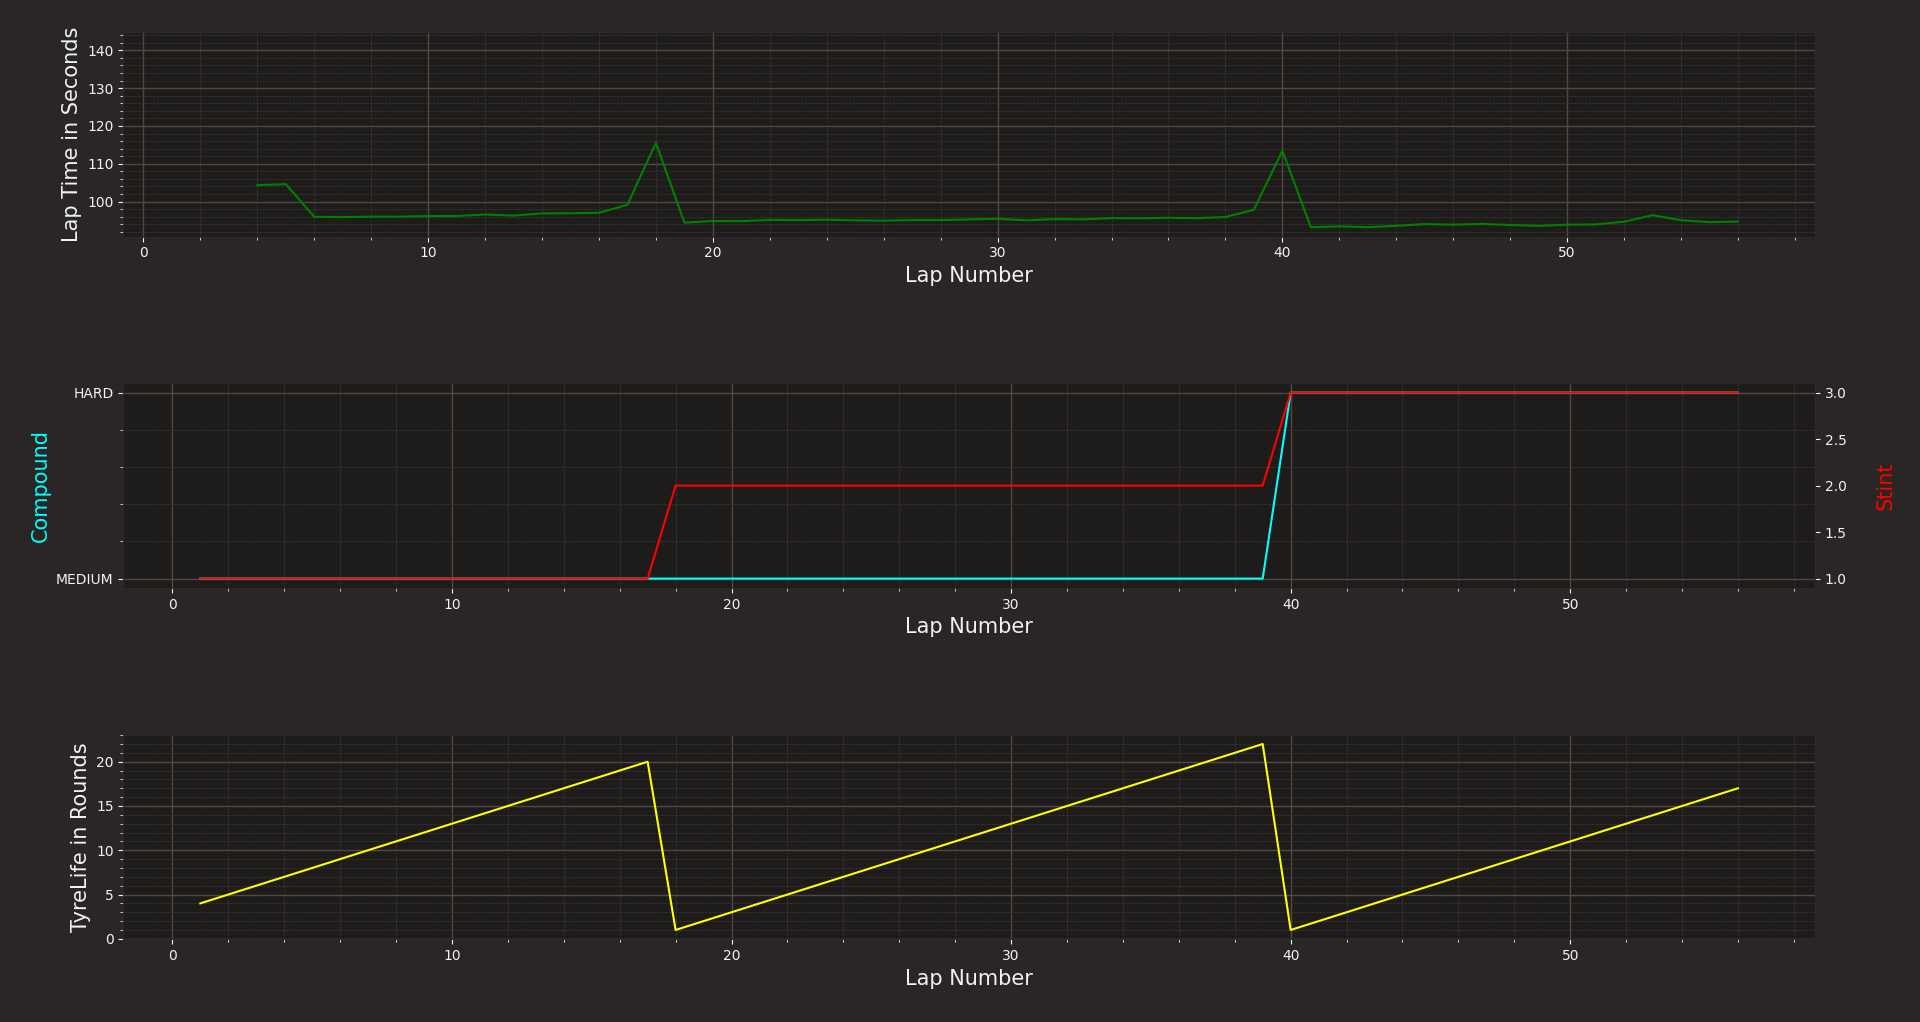
\includegraphics[scale=0.33]{Studienarbeit_F1/images/ver_race_data_example.png}
    \caption{Renndaten für Max Verstappen, Bahrain Grand Prix 2021}
    \label{fig:race_data_2021_1_VER}
\end{figure}

In Abbildung \ref{fig:race_data_2021_1_VER} ist ein beispielhafter Datensatz, welcher als Datengrundlage zur Generierung der Modelle dient, abgebildet. Hierbei sind die gefahrenen Rundenzeiten über das gesamte Rennen abgebildet, sowie die verwendeten Reifen und deren Grad der Abnutzung über die Anzahl an Runden, welche der Reifen bereits bestritten hat. Dieser Datensatz beschreibt das Rennen vom Fahrer Max Verstappen in Bahrain im Jahre 2021. Entsprechend unserer Datengrundlage können wir unsere Modelle auf die Kombination all dieser zur Verfügung stehenden Datensätze aufbauen. Über den Zeitraum von 2018 bis 2021 mit etwa 21 Rennen pro Saison und durchschnittlich 18 Autos, welche das Ziel erreichen, entspricht dies etwa 1500 nutzbare Datensätze zur Generierung der Modelle.




\subsubsection{Generierung der Modelle}\label{sec:gen_models}
% Fully corrected
% Guck ma Statistik, vllt n bissl Regression etc -> Alos von Daten zu Modellen beschreiben
Um aus der aufgebauten Datengrundlage effektiv Modelle zur Beschreibung der diversen Reifenmischungen generieren zu können, bedurfte es zunächst eine Möglichkeit, die Daten zielgerichtet auszulesen. Für diese Aufgabe wurde ein eigener \gqq{Query Handler} geschaffen, welcher es erlaubt, einzelne Teilmengen aus den gesamten Daten herauszufiltern. Dieser erlaubt wie schon beim Akquirieren der Daten nach dem gefahrenen Jahr, dem Fahrer und der Reifenmischung einzugrenzen. Zusätzlich ist in diesem Schritt aber wichtig, die gefundenen Stints nach einer Mindestlänge zu filtern, um somit nur aussagekräftige Datensätze zu erhalten. Dies bedeutet, dass beispielsweise alle Stints von \gqq{Hard} Reifen, welcher unter 10 Runden betrugen, nicht mit ausgewertet werden sollten, da dieser Zeitraum zu kurz ist, um das Verschleißverhalten daraus abzuleiten bei einer Lebensdauer des Reifen von etwa 50 Runden bei einer Rundenzeit von etwa 80 Sekunden. Die Lebensdauer des Reifens sollte hierbei nochmals in Kontext gesetzt werden. So beschreibt diese Nomenklatur nicht den Rahmen, in welchem der Reifen von einem neuwertigen Zustand übergeht zu einem Reifenplatzer. Vielmehr beschreibt die Lebensdauer das nutzbare Fenster, in welchem der Reifen im Rennbetrieb eingesetzt werden sollte. Dies bedeutet ein Reifen, welcher eine Lebensdauer von etwa 50 Runden besitzt, könnte bei Bedarf auch 20 weitere Runden durchhalten, aber in dieser Zeit werden die Rundenzeiten dramatisch schlechter und das Risiko eines Reifenplatzers steigt stetig, was in jedem Fall zu vermeiden ist. Somit bezeichnet der Begriff der Lebensdauer den Rahmen, in welchem der Reifen ein vorhersehbares und sicheres Verhalten besitzt und dabei kompetitive Rundenzeiten liefern kann.\\\\
Um eine möglichst repräsentative Auswertung für jede Art von Reifen durchzuführen, sollen alle relevanten Datensätze zu einem gültigen Modell zusammengefasst werden. Die somit ausgewählte Teilmenge der Datensätze kann nun aus verschiedensten Faktoren bestehen, welche zunächst eine Vergleichbarkeit der Daten untereinander verhindern. Grundlegend sind die Rundenzeiten meist auf verschiedenen Strecken gefahren, welche somit die Reifen in anderem Umfang strapazieren, aber auch entsprechend mehr oder weniger Zeit in Anspruch nehmen. Weitere Einflussfaktoren der Rundenzeit sind durch die Diversität der Autos selbst und das Können der einzelnen Personen am Steuer der Fahrzeuge gegeben. Um eine Vergleichbarkeit der Daten sicherzustellen, müssen die einzelnen Rundenzeiten der Stints auf eine Referenzzeit normiert werden. Dies schließt somit alle bisherigen Einflussfaktoren aus den Zeiten aus und belässt lediglich den Verlauf der Rundenzeit über den Zeitraum des Stints. Dieser Verlauf besitzt eine direkte Abhängigkeit zum Verschleiß des Reifens und kann somit als Basis des Modells genutzt werden.
\\
Methodisch erfolgt die Normierung durch die Auswahl einer einzelnen Rundenzeit im Stint, in unserem Falle die erste Runde des Stints. Im folgenden Schritt wird der Quotient aus Referenzzeit und der ausgewählten Rundenzeit berechnet und dann auf alle anderen Rundenzeiten des Stints angewendet, um diese somit einzelnen und unabhängig zu anderen Stints der Teilmenge zu normieren. 
\begin{equation}
    L_{nom} = L * \frac{L_{ref}}{L_{stint}}
\end{equation}
Die genutzte Referenzzeit wurde auf 80 Sekunden gewählt, da dies ungefähr der durchschnittlichen Rundenzeiten in der Formel 1 über eine Saison entspricht und somit anschließend in einer Rennlänge von etwa 70 Runden resultiert. Dies bietet auch den Vorteil, dass die KI später 70 Entscheidungen pro Rennen treffen muss und damit der Lernerfolg pro Rennen größer sein sollte als bei der Verwendung einer größeren Referenzrundenzeit. Die oben genannte Rennlänge in der Formel 1 beschreibt die Anzahl der Runden, welche zu absolvieren sind und abschließend etwa einer gesamten Renndauer von 90 Minuten entsprechen sollen.
\\
Anschließend wird aus jedem der gesammelten Datensätze, welche der gewünschten Teilmenge entsprechen und zu diesem Zeitpunkt normiert sind, ein Modell errechnet, welches perfekt den einzelnen Datensatz beschreibt. Die Errechnung der Modelle ist dabei auf einer Analyse über die Stintlänge von 0 bis Ende des Stints in Anzahl der Runden und der entsprechenden Rundenzeit pro Runde gegeben. Zur Approximation der Modelle wird die Polynominal Regression auf Basis des \gqq{Least Squares}-Ansatzes genutzt, welche in \ref{sub: polynominal_regression} näher beschrieben wird. Dies bedeutet, dass bei einer Menge von $x$ Daten auch $x$ Modelle generiert werden. Danach werden die einzelnen Modelle dann über die Verrechnung der einzelnen Parameter zusammengefasst, um somit ein einzelnes Modell zu generieren, welches die gewünschte Teilmenge vollständig repräsentiert. Das Zusammenfassen der einzelnen Parameter erfolgt hierbei über das arithmetische Mittel oder wahlweise dem Median. Wobei sich das arithmetische Mittel durch seine glättende Eigenschaft besser eignet.
\\\\
Das Modell zur Betrachtung der individuellen Leistung eines Fahrzeuges in Kombination mit dem Fahrer soll dabei auf der Auswertung zwischen dem schlechtesten Fahrer im schlechtesten Auto und dem besten Fahrer im besten Auto erfolgen. Hierbei ist das Kernproblem, dass der Fahrer aus den Daten heraus nicht vom Fahrzeug getrennt betrachtet werden kann, da nur zwei Fahrer im Feld das gleiche Fahrzeug besitzen. Somit kann nur eine Aussage zwischen diesen Fahrern getroffen werden. Ein Vergleich des fahrerischen Könnens über das ganze Feld hinweg ist wissenschaftlich schwer realisierbar, da die Ergebnisse der einzelnen Fahrer immer direkt mit der Leistung des Fahrzeuges korrelieren.\\
Um dennoch ein Modell zu generieren, welches uns die zeitliche Differenz pro Runde in Kontext zur Fahrzeugleistung und Fahrerleistung setzt, werden repräsentative Datensätze ausgewählt und wie beim Reifenmodell auf eine Referenzrundenzeit von 80 Sekunden normiert, um anschließend den mittleren zeitlichen Unterschied pro Runde zwischen Datensätzen verschiedener Leistung zu generieren und daraus ebenfalls mit Hilfe der Polynominal Regression ein aussagekräftiges Modell zu erstellen. Dieses soll dann die einzelnen Parameter der Leistung des Fahrzeuges und des Fahrers als Summe zu einem Zeit-Delta pro Runde korrelieren. Diese Parameter sind im Simulator als Werte zwischen $[0,1]$ gegeben mit $1$ für die beste Leistung. Entsprechend soll das Modell einem Fahrzeug, welches eine kombinierte Leistung von $2$ besitzt, keine zusätzliche Zeit pro Runde aufaddieren.


\subsection{Künstliche Intelligenz}
\label{künstliche_Intelligenz}
Auf Basis des initial entwickelten Simulators wurden die ersten Versuche der KI-gestützten Optimierung der Rennstrategie unternommen. Ziel dieser Bemühungen war es, für einen bestimmten Akteur des Rennens für jeden Zeitschritt der Simulation eine Aktion abzuleiten, die abhängig vom momentanen Rennzustand die Position des gewählten Fahrers verbessert. Diese Anforderungen resultieren in den folgenden, zu lösenden Subproblemen:
\begin{enumerate}
    \item Evaluierung von geeigneten KI-Algorithmen
    \item Integration eines Prototypen in die existierende Architektur
    \item Optimierung der KI-Parameter
    \item Evaluierung der Performance
\end{enumerate}
Im Weiteren werden die verfolgten Ansätze zur Bewältigung dieser Hürden erläutert.

\subsubsection{Evaluierung geeigneter KI-Algorithmen}
Um eine Optimierung des Renngeschehens realisieren zu können, ist es vonnöten, den Zustand einzelner Akteure in eine der vier möglichen Aktionen umzusetzen. Drei dieser Optionen beinhalten einen Pitstop mit verschiedenen Reifen, während die übrige Möglichkeit das unveränderte Fortfahren repräsentiert. Benötigt wird folglich eine Abbildung, die sowohl die Wahl des zu optimierenden Akteurs sowie alle erhältlichen Daten des Simulators als Eingabe nimmt und diejenige der 4 möglichen Handlungen, welche die Position des gewählten Akteurs optimiert, zurück gibt. Während die Größe der Eingabe- und Ausgabevektoren mittels der bereits beschriebenen Perzeptron-Technik der neuronalen Netze realisiert werden kann, ist bei der Verwendung eines solchen Ansatzes fragwürdig, inwiefern die Zuordnung des korrekten Fahrers einfach durch das Nutzen eines zusätzlichen Eingabeparameters geschehen kann. Diese Assoziation müsste aus dem Lernprozess des Netzes hervorgehen, jedoch ist keineswegs garantiert, dass solch ein Effekt auftritt. Um zu garantieren, dass diese Anforderung folglich im finalen Algorithmus realisiert wird, sollten äußere Anforderungen dieser Form nicht als durch den Lernprozess zu beseitigende Freiheitsgrade der KI repräsentiert werden, sondern nach Möglichkeit durch die architektonisch bedingten Grenzen forciert werden. Konkret bedeutet dies, dass eine Assoziation des gesteuerten Fahrers und der KI im ersten Versuch nicht mittels der Eingabeparameter geschieht.\\
Eine weitere Problematik des skizzierten Ansatzes stellt die Frage des Lernprozesses dar. Die beschriebene Technik lässt sich dem überwachten Lernen zuschreiben und benötigt für den Lernprozess die für die Anwendung \gqq{korrekten} Ausgabevektoren. Die optimalen Simulatoreingaben für die Positionsoptimierung zu jedem Zeitschritt zu ermitteln ist jedoch gerade die Motivation für die Entwicklung des Netzes, folglich greift der Ansatz des klassischen neuronalen Netzes allein für die vorliegende Problematik zu kurz und muss erweitert werden.\\
Die Behandlung der vorliegenden Problematik lässt sich vereinfachen, indem die Umgebung des Simulators als Spiel verstanden wird. Durch das Ausführen einer Aktion wirkt der Agent auf sein Umfeld ein und produziert in jeder Runde einen neuen Zustand. Am Ende des Rennens kann eine Bewertung des Spielers basierend auf seiner Position erfolgen. Es ist daher naheliegend, hier auf die existierenden Techniken beim maschinellen Lernen von einfachen Spielen zurückzugreifen. Die am weitesten verbreiteten Verfahren hierbei lassen sich unter dem Begriff \gqq{reinforcement-learning} (RL) zusammenfassen. Eine Übersicht einiger Techniken findet sich in \cite{reinforcement_learning_study}. Gemeinsames Ziel dieser Ansätze ist es, einen Lernprozess für derartige Probleme zu beschreiben, bei denen ein sogenannter \gqq{Agent} durch die Interaktion mit seiner Umgebung ein Steuersignal in Form einer Belohnung erhält, das bestimmte Verhaltensweisen fördern und andere behindern soll. \cite{reinforcement_learning_study} nennen für die Charakterisierung eines RL-Problems die folgenden beschreibenden Eigenschaften: 
 \begin{itemize}
     \item Eine diskrete Menge von Umgebungszuständen
     \item Eine diskrete Menge von vom Agenten zu tätigenden Aktionen
     \item Eine Menge von Zahlen als Belohnungen dienen
 \end{itemize}
 Um diese Punkte für den Rennsimulator herzustellen wird lediglich noch eine Funktion zur Ausschüttung von Belohnungen basierend auf dem Zustand benötigt.\\
 Die verschiedenen Ansätze des reinforcement-learning lassen das Optimieren der Leistung eines maschinellen Spielers in einer breite Klasse an Spielumgebungen zu. Beispielhaft sind Erfolge bei verschiedenen Atari-Spielen wie in \cite{atari_deep_reinforcement_learning} zu nennen oder das Meistern des komplexen Spieles Go durch Googles AlphaGo zero\footnote{\cite{alpha_go}}. Um eine für die vorliegende Anwendung zielführende Technik zu finden werden zunächst einige RL-Ansätze vor dem Hintergrund des Rennsimulators beleuchtet.


\subsubsection{Q-learning und Deep-Q-learning}
Allgemeines Ziel des Reinforcement-Learnings ist es, den Erwartungswert der kumulierten Belohnungen zu maximieren. Ein grundlegendes Modell der gesamten erhaltenen Belohnungen \(Q\) in Abhängigkeit eines Zustands \(s\) und einer Aktion \(a\) lässt sich wie folgt definieren:
\[Q(s, a) = r + Q(s')\]
Wobei \(r\) die initial ausgeschüttete Belohnung darstellt und \(Q(s')\) die gesamten zukünftigen Belohnungen ab dem nächsten Zustand bei Ausführung einer bestimmten Aktion repräsentiert. Ein Q-Learning Algorithmus lernt die Q-Werte für jedes Tupel aus Zustand und Aktion näherungsweise zu bestimmen und folglich diejenige Aktion zu ermitteln, die den Maximalwert liefert. Es resultiert ein Pfad aus Handlungen des Agents, der eine nach dem Lernprozess optimale Strategie abbildet. Abhängig von der zu erlernenden Aufgabe resultieren verschiedene Ansätze beim Schätzen des Q-Wertes in unterschiedlich effektiven Lernprozessen und Strategien. Aufgrund der inexakten Natur des von einem Algorithmus gelieferten Q-Wertes ist es opportun, die weiter in der Zukunft liegenden und damit ungenauer bestimmbaren Belohnungen weniger stark zu gewichten als solche, die mit geringer Varianz ermittelbar sind. Im Weiteren kann die mathematische Darstellung zusätzlich insofern spezifiziert werden, dass der beschriebene Algorithmus immer diejenige Aktion wählt, die im maximalen Q-Wert mündet. Diese Tatsachen lassen sich wie folgt in eine verbesserte mathematische Beschreibung umwandeln:
\[Q(s, a) = r + \gamma \cdot max(Q(s'))\]
Hierbei liegt \(\gamma\) zwischen 0 und 1 und verwirklicht die geringere Sicherheit bei entfernten Werten, wie durch das rekursive Einsetzen der Definition des Q-Wertes evident wird.\\
Die Subtypen des Q-learning unterscheiden sich explizit in der Art des Lernprozesses und damit der Bestimmung von Q. Für Probleme mit einer geringen Anzahl an diskreten Zuständen und Aktionen wird eine sogenannte \gqq{Q-Table} verwendet. Dieser Ansatz lässt sich im Wesentlichen als \gqq{Bruteforce} Methode zur Ermittlung des Wertes aller möglichen Zustandstransitionen charakterisieren und ist folglich nicht im Kontext der hier vorliegenden Vielzahl an Zuständen realisierbar.\footnote{vgl. \cite{general_Q_learning}}\\
Das in der Praxis gängige Verfahren zur Kompression der Vielzahl an vorliegenden Zustands- und Aktionstupeln ist der Einsatz eines neuronalen Netzes als prädiktionsliefernde Instanz. Konkret bedeutet dies, dass zuvor ein Netz die Belohnungen für verschiedene Zustände exemplarisch durchläuft und schlussendlich in Folge dieser Beispiele die zu erwartenden Belohnungen auch ohne die Kenntnisse über alle Zustände des Systems näherungsweise bestimmen kann. Dieses Verfahren wird als \gqq{Deep-Q-Learning} bezeichnet. Die zentrale Schwierigkeit dieses Ansatzes stellt das Trainieren des Netzes dar. Wie bereits erwähnt ist ein klassisches neuronales Netz eine Technik des überwachten Lernens, dies bedeutet, dass die Daten zum Trainieren in solch einer Form vorhanden sein müssen, dass zu jedem Beispiel der korrekte Output vorhanden sein muss. Die Eingabe des Umgebungszustandes auf die insgesamt zu erwarteten Belohnungen bei der Ausführung aller möglichen Aktionen abzubilden, ist jedoch nicht trivial. Um den Lernprozess zu ermöglichen wird für die beim Deep-Q-learning verwendeten Netze\footnote{Diese werden als \gqq{Deep-Q-Networks} (DQNs) bezeichnet} die initial bei der Zustandstransition ausgeschüttete Belohnung in Kombination mit den durch das Netz selbst berechneten, zu erwartenden Belohnungen in Folge des resultierenden Zustands verwendet, um die Performance des Netzes, also den Fehler in der Ausgabe, zu bewerten. Um dies zu verdeutlichen, wird der Lernprozess im Folgenden schrittweise illustriert:
% TODO Quellennachweise für den Algorithmus
% Ist das so verständlich oder sollte das eventuell Pseudocode sein?
\begin{enumerate}
    \item Netzinitialisierung : Zufällige Gewichte liefern anfangs für jede Eingabe zufällige Ausgaben
    \item Der Agent erhält eine Prädiktion von Belohnungen des Netzes in Form des Vektors \(Q(S)\) für den momentanen Zustand \(S\) und führt diejenige Aktion aus für die der Eintrag \(Q(S)\) maximal ist
    \item Der Agent beobachtet in Folge der getätigten Aktion \(a\) eine Belohnung \(r\) und speichert diese mit dem neuen Zustand \(S'\) und dem initial vom Netz erhaltenen Vektor an erwarteten Belohnungen ab
    \item Mithilfe von \(r\) und \(Q(S')\) wird ein Belohnungsvektor \(Q'(S)_a\) mit \gqq{korrekterem} Eintrag für die getätigte Aktion berechnet.
    \item Der Fehler aus der Abweichung von \(Q(S)\) und \(Q'(S)_a\) berechnet, wobei beide Vektoren sich lediglich im \(a\) repräsentierenden Index unterscheiden
    \item Wiederhole die Schritte ab 2. für alle Trainingsbeispiele
\end{enumerate}
Die Berechnung des korrigierten Eintrags des Belohungsvektors aus Schritt 4 geschieht wie folgt: 
\[Q(S)_a = r + \gamma \cdot max(Q(S'))\]
Die Bestimmung der Belohnungen des nächsten Zustandes geschieht demnach durch das zu trainierende Netz selbst. In jedem Lernschritt wird der betroffene Eintrag also nur durch die erhaltene Belohnung in die korrekte Richtung geführt.\footnote{vgl. \cite{atari_deep_reinforcement_learning} S.5} Um die Effektivität des Algorithmus zu steigern, betont Mnih, dass es hierbei zwei Netzwerke identischer Topologie geben muss, um die initiale Berechnung von Q-Werten und die Berechnung von den gewünschten Ziel-Q-Werten zu entkoppeln. Die Gewichte des Prädiktionsnetzes werden hierbei im Lernprozess optimiert und in einem festen Intervall auf das Zielnetzwerk kopiert.

\subsubsection{Implementierung eines DQN-Prototyps}
Um die beschriebene Technik erfolgreich umzusetzen, wurde zunächst ein Prototyp mit möglichst simplem Aufbau in die existierende Architektur des Simulators eingebettet. Ziel hierbei waren zunächst die Lauffähigkeit eines neuronalen Netzes und das sichtbare Anlernen von Belohnungen zu verifizieren und darauf folgend die Effektivität des Ansatzes bewerten zu können, um weitere Entscheidungen bei der Optimierung zu treffen.\\
Der geplante Ablauf einer Lernepisode lässt sich in Abbildung \ref{fig:race_ai_learning_episode} nachvollziehen.
\begin{figure}[ht]
    \begin{center}
        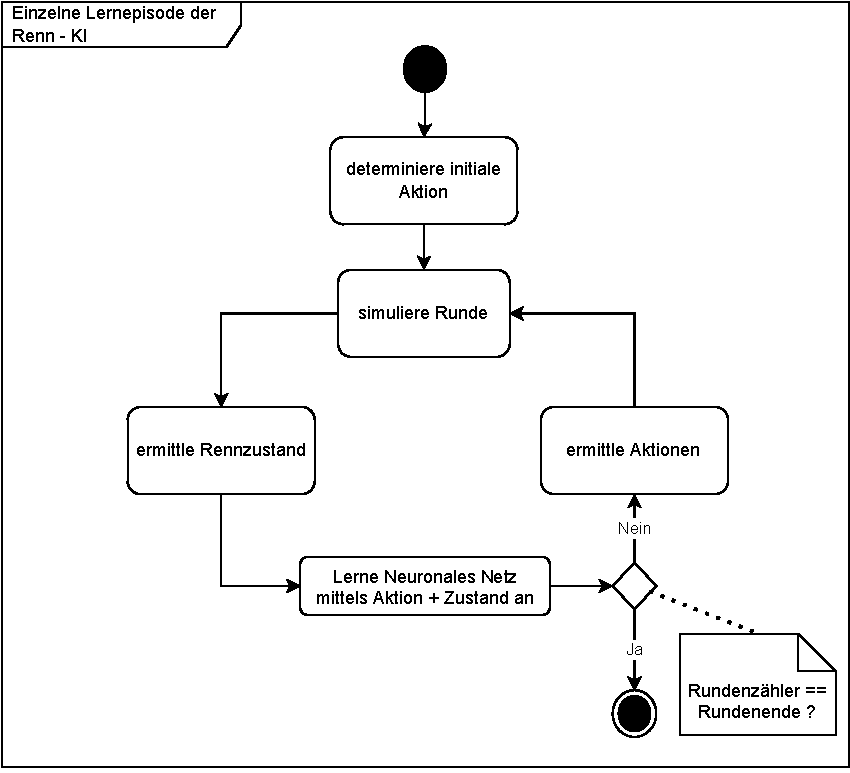
\includegraphics[]{Studienarbeit_F1/images/diagrams/race_ai_episode.pdf}
    \end{center}
    \caption{Geplanter Ablauf einer Lernepisode des DQN}
    \label{fig:race_ai_learning_episode}
\end{figure}
Einen wesentlichen Unterschied zu den bereits implementierten Funktionalitäten stellt die Rolle des Rennsimulators hier dar. Anstatt ein ganzes Rennen in einer Schleife zu simulieren, ist es für die KI-Entscheidung nötig, das Geschehen rundenweise verfolgen zu können. Opportun in diesem Kontext ist es, eine Funktion zu haben, die einen Rennzustand und die Aktionen der einzelnen Fahrer als Parameter nimmt und einen neuen Zustand zurückgibt. Der KI-Agent ist insoweit von den inneren Funktionsweisen des Simulators entkoppelt, dass verschiedene Funktionen den gesamten Rennzustand in die für das Lerngeschehen relevanten Werte umwandeln.
Explizit benötigt werden die folgenden Größen:
\begin{itemize}
    \item Die Belohnung für eine Aktion
    \item Der Eingabevektor für das neuronale Netz
\end{itemize}
In erster Iteration wurde sich bei der Eingabe des Netzes für die Anzahl der übrigen Runden bis zum Ende des Rennens, sowie die prozentuale Abnutzung des momentanen Reifens des der KI zugewiesenen Autos entschieden. Die Belohnungsfunktion besitzt zwei verschiedene Definitionen : einerseits wird für alle Runden außer der letzten eine Belohnung in Abhängigkeit der Veränderung des Abstands zum schnellsten Fahrer ausgeschüttet, andererseits wird am Ende des Rennens der finale Rückstand zum schnellsten Fahrer als negative Belohnung verteilt. Befindet sich der KI-Fahrer an erster Stelle, so wird der Abstand zum zweitschnellsten Auto zusätzlich auf die Belohnung addiert. Um die kumulierte Belohnung zu maximieren muss somit die Rundenzeit minimiert werden.\\
Die initiale Architektur des Netzes spiegelt die geforderte Simplizität des Prototypen wieder. Basierend auf dem gewählten Eingabevektor besteht die erste Schicht lediglich aus zwei Neuronen. Die Ausgabeschicht spiegelt die Anzahl der möglichen Aktionen wieder, demnach ist diese hier vier Neuronen breit. Nach Goodfellow\footnote{Vgl. \cite{goodfellow_deep_learning} S.422 f} ist die Wahl der sonstigen Hyperparameter des Netzes wie der Anzahl der Schichten und deren Größe ein problemspezifischer Prozess, der bestenfalls mittels eines bereits funktionsfähigen Prototypen durchlaufen wird. Als erste Näherung wurde sich aufgrund der geringen Komplexität der Eingabe für eine versteckte Schicht entschieden. Die Neuronenanzahl in dieser wurde mit 400 wissentlich zu hoch angesetzt, da vermutet wurde, dass die höhere Anzahl zwar zu einem langsameren Lernprozess führt, aber die zu prüfende Funktionsfähigkeit des Ansatzes trotzdem observierbar wird. Die Lernrate wurde nach ähnlicher Methode mit einem Initialwert von \(10^{-5}\) festgesetzt. Hierbei wurde vermutet, dass aufgrund der von Goodfellow betonten Wichtigkeit dieses Parameters eine Nachjustierung erfolgen müsste.\\
Weitere wichtige Entscheidungen beim Design des Netzes sind die Wahl der Aktivierungsfunktion und der Fehlerfunktion. Aus den bereits in Kapitel \ref{künstliches_neuron} beleuchteten Aktivierungsfunktionen scheint die ReLU-Funktion für die vorliegenden Eingaben und Ausgaben am besten geeignet. Die Eingabegrößen sind stets positive Zahlen mit leicht unterschiedlichen Wertebereichen und die gewünschten Ausgaben reichen von \(-\infty\) bis \(\infty\), was sich leicht durch Anwendung von ReLU in allen Schichten außer der letzten erreichen lässt. Für die finale Schicht wird als Aktivierungsfunktion die Identitätsfunktion verwendet, um auch den negativen Wertebereich abzudecken.
Als zu minimierende Kostenfunktion des Netzes wurde sich für die mittlere quadratische Abweichung des Zielwertes vom momentanen Wert der Ausgabe entschieden, da diese einen intuitiv nachvollziehbaren Zusammenhang zwischen der Netzausgabe und
dem Fehler herstellt, was die Evaluierung des Netzes durch die bessere Nachvollziehbarkeit der einzelnen Schritte vereinfacht.
Eine zusammenfassende Übersicht der initialen Konfigurationen im Weiteren relevanter Parameter als Python-Code findet sich in Listing \ref{lst:params}.
Bezüglich des Lernprozesses ist zu ergänzen, dass die Erfahrungen in Form von Tupeln aus Zustand, Aktion, Belohnung und folgendem Zustand den Erfolg des Lernens bestimmen. Um eine optimale Strategie zu entwickeln, ist es somit nötig, dem Agenten möglichst viele verschiedene Erfahrungen zukommen zu lassen.
\begin{figure}
\begin{lstlisting}[label={lst:params}, caption={Initiale Konfiguration von KI-Parametern}]
   learning_rate = 1e-5 
   gamma = 0.999
   episodes = 3000
   layer_sizes = [2,400,4]
   memory_batch_size = 500
   target_prediction_update_interval = 500
   
   # KI-Strategie
   epsilon = 1
   epsilon_decay = 0.001
   epsilon_min = 0.01
\end{lstlisting}
\end{figure}
Gleichzeitig führt eine solche Erkundung der Umgebung bei fixierten Lernepisoden dazu, dass die KI weniger Erfahrungen bei den bereits \gqq{erprobten} Strategien sammelt. Diese Balance zwischen der Erkundung neuer Strategien und der Ausnutzung derer, die nach momentanem Stand die optimale Belohnung liefert, ist als \gqq{Exploration vs. Exploitation} bekannt und muss für jedes RL-Problem gefunden werden. Um im Kontext der Renn-KI einen verbesserten Lernprozess zu provozieren, wird eine sogenannte \(\epsilon\)-greedy Policy zusammen mit Experience-Replay verwendet. \(\epsilon\)-greedy bedeutet, dass eine Variable names Epsilon verwendet wird, um die Wahrscheinlichkeit anzugeben, dass eine Aktion nicht infolge der Netzwerk-Prädiktion gewählt wird, sondern zufällig ausgeführt wird. Dieser Wert startet bei 1 und wird in jeder Episode durch den Wert von epsilon\_decay vermindert bis er einen Mindestwert erreicht. Dieses Schema ergibt eine linear abnehmende Häufigkeit an zufällig gewählten Aktionen und hilft der KI besonders in der Anfangsphase die optimale Strategie zu finden.\footnote{Vgl. \cite{deep_reinforcement_learning} S.14}\\
Experience-Replay bezeichnet das Speichern von Erfahrungen und das damit verbundene, zusätzliche Lernen aus den Selbigen. Vorteile sind die Verfügbarkeit von mehr Trainingsdaten allgemein, deren statistische Dekorrelation durch zufälliges samplen\footnote{Vgl. \cite{dqn_implementation} S.3}, sowie die Prävention von Effekten, die dem Vergessen von initialen Trainingserfolgen durch das Erfahren selektiver Trainingsdaten bei der Verfolgung einer optimalen Strategie ähneln. Ein derartiges Phänomen wird als \gqq{catastrophic forgetting} bezeichnet und kann beispielsweise durch das stetige erneute Lernen aus den früheren \gqq{Katastrophen} verhindert werden.\footnote{Vgl. \cite{experience_replay_continual_learning} S.1} Ebenso für die Mitigation dieses sich negativ auswirkenden Effektes eignet sich das alleinige Verwenden der Netzparameter, die die beste Performance liefern.

\subsubsection{Evaluierung und Anpassung des Prototypen}
Um die Funktionsfähigkeit der dargelegten Architektur zu prüfen, wurde zunächst der Lernprozess in Form von der Größe des Fehlers der Ausgabevektoren der KI und der Belohnungen zum Ende des Rennens in einem Logfile abgelegt. Hierdurch konnte schnell erkannt werden, dass der Wert der Lernrate stark reduziert werden musste. Nach einigen Episoden ergaben sich nämlich so große Werte für den Gradienten, dass die resultierenden Anpassungen der Gewichte den Wertebereich dieser überschritten, was im Log zu Einträgen mit NaN führte. Eine Lernrate von rund \(10^{-9}\) ließ diese Effekte verschwinden und lieferte nach 10 Testläufen die besten Ergebnisse verglichen mit noch kleineren Werten. Ebenfalls erkennbar wurde, dass die sehr simple Architektur mit einer hidden-Layer Schwierigkeiten hatte, die nicht stetigen Übergänge zwischen der Belohnung pro Runde und der Belohnung am Ende des Rennens zu lernen. Dies äußerte sich in Ausreißern des Fehlers am Ende jedes Rennens, welche unabhängig von der Performance der KI auftraten. Verstärkt wurden diese durch das Verwenden der mittleren quadratischen Abweichung als Fehlerfunktion, die derartige Extremwerte zusätzlich gewichtet. Grundsätzlich ist ein Auftreten großer Fehlerwerte am Ende des Rennens gewünscht, da hier der größte Lerneffekt auftreten sollte. Ein angelerntes Netz sollte derartige Sprünge jedoch nicht aufweisen. Um das Problem zu lösen, wurde zunächst der gesamte Wertebereich der Belohnungsfunktion verkleinert. Diese Änderung resultiert in einer verkleinerten Streuung der Belohnungen über die Zeit und verkleinert die Ausreißer erheblich. Jedoch musste die Lernrate infolge der nun verringerten Fehlerwerte wieder erhöht werden. Um einen effizienteren Trainingsprozess zu erreichen, wurde die Anzahl der Neuronen in der versteckten Schicht zusätzlich auf 30 reduziert, da hier keine Verschlechterung wahrgenommen werden konnte. Mit diesen Änderungen gelang es, einen KI-Agent zu trainieren, der sichtliche Lernerfolge erzielt und zuverlässig eine bessere Platzierung als die initiale, untrainierte KI erreichen kann. Die Abbildungen \ref{fig:AI_initially_trained_soft} und \ref{fig:AI_initially_trained_hard} zeigen diesen Lernfortschritt in Form der gesammelten Belohnungen am Ende des Rennens nach den durchlaufenen Episoden für zwei Durchläufe bei identischer Konfiguration.
Auffallend bei Abbildung \ref{fig:AI_initially_trained_soft} ist, dass die KI nach einer anfänglichen Einfindungsphase in ein oszillierendes Schema von Strategiewechseln verfällt. Das Muster resultiert daraus, dass die KI lernt, dass ein besseres Ergebnis dadurch erzielt werden kann, einen Reifen weniger oft zu wechseln. Folglich nähert sich die Lebenszeit des Reifens immer mehr den 0\%, ab welchen die Rundenzeit stark zu steigen beginnt. Dies führt zu einem großen Fehler in der Schätzung des neuronalen Netzes und demnach auch in einer großen Anpassung der Gewichte. Die vorherige Strategie wird damit als schlechter bewertet und der Agent weicht auf diejenigen Aktionen aus, die nun die besten Belohnungen liefern. Diese neue Strategie liefert im Mittel jedoch schlechtere Resultate als die Alte, somit kehrt der Agent nach einigen Episoden wieder zur Ausgangsstrategie zurück.
\begin{figure}
\begin{center}
    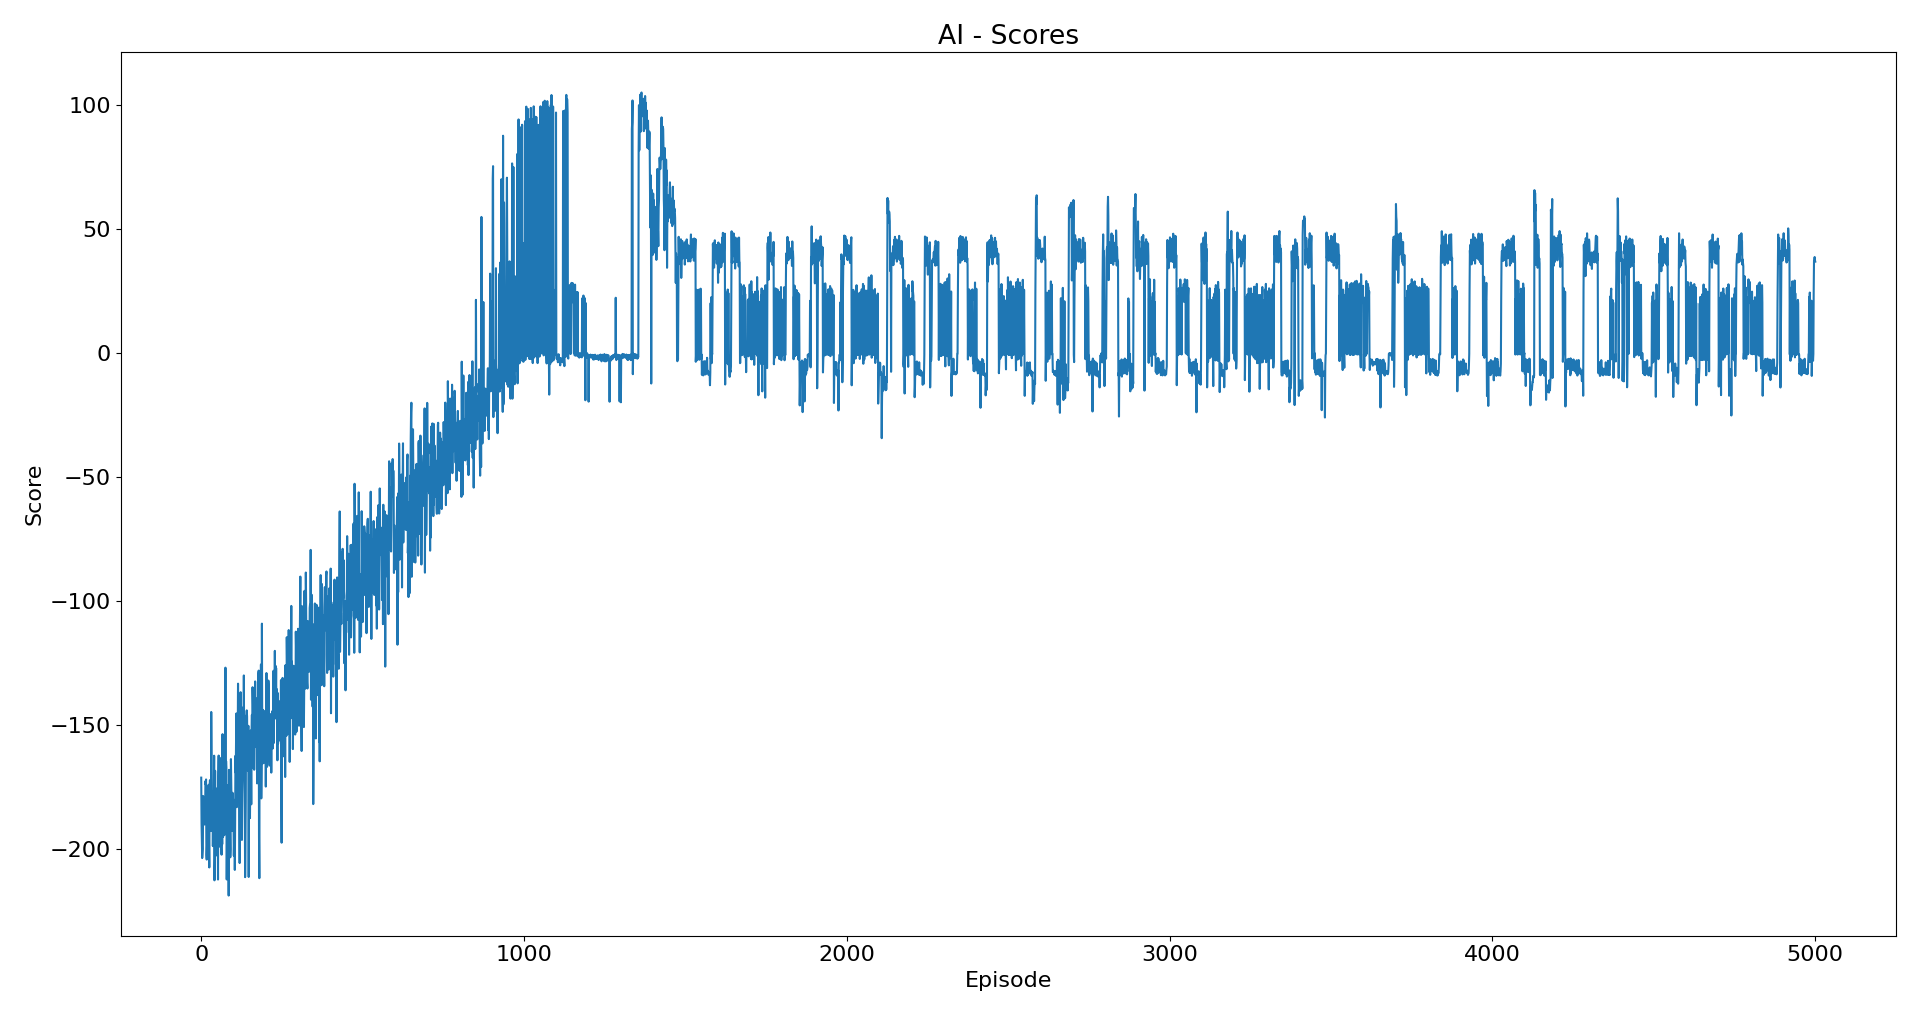
\includegraphics[scale=0.33]{Studienarbeit_F1/images/scores_5000eps_soft.png}
    \caption{Summierte Belohnungen nach jeder Lernepisode über 5000 Episoden. Eine Lernepisode repräsentiert ein Rennen mit 70 Runden. Die ersten 1000 Episoden werden durch die Epsilon-Policy dominiert.}
    \label{fig:AI_initially_trained_soft}
\end{center}
\end{figure}
\begin{figure}
    \centering
    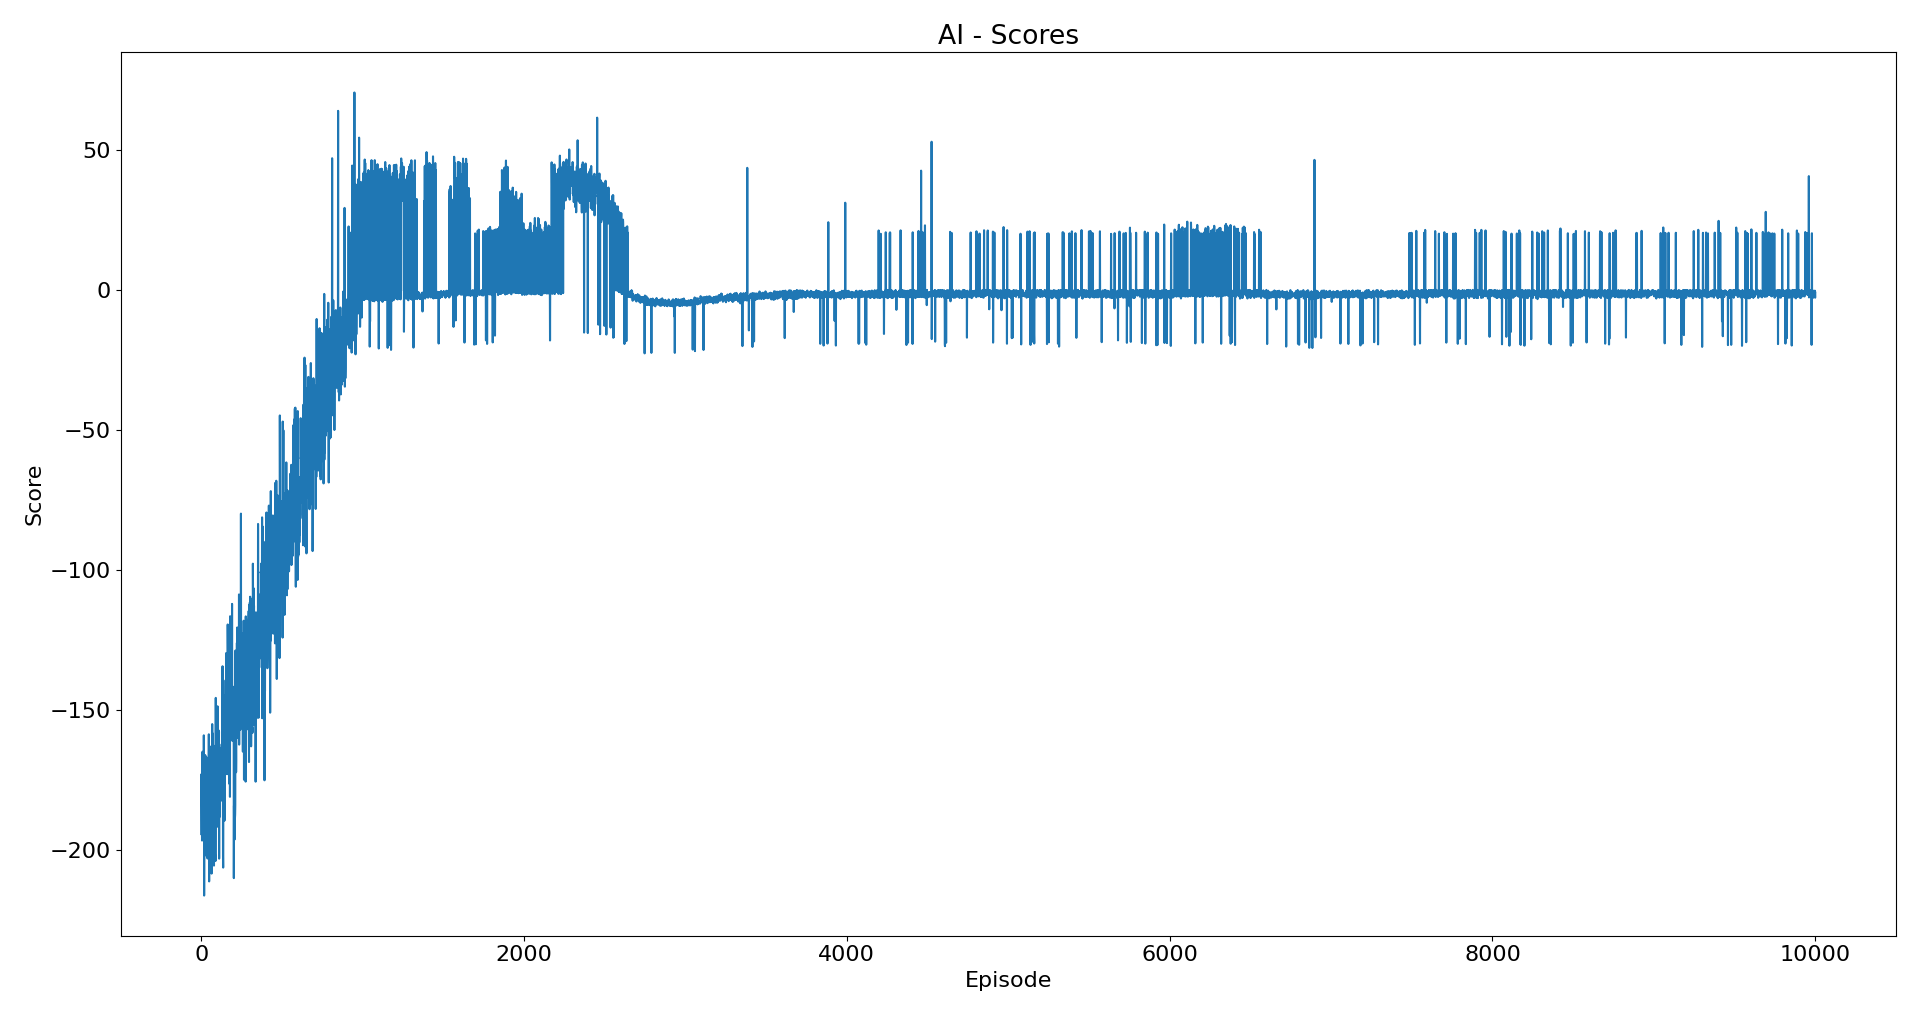
\includegraphics[scale=0.33]{Studienarbeit_F1/images/scores_10000eps_hard.png}
    \caption{Summierte Belohnungen nach jeder Lernepisode über 10000 Episoden. Es dominiert bei gleicher Konfiguration wie in Abbildung \ref{fig:AI_initially_trained_soft} eine unterschiedliche Strategie.}
    \label{fig:AI_initially_trained_hard}
\end{figure}
Zusätzlich für einen suboptimalen Lernprozess spricht der im Vergleich in Abbildung \ref{fig:AI_initially_trained_hard} gezeigte Verlauf. Bei einer idealen Erkundungsstrategie des Agenten ist zu erwarten, dass jeder Trainingslauf bis auf geringe Unterschiede diejenige Strategie hervorbringt, die die optimalen Resultate erzielt. Es folgt, dass der hier verfolgte Ansatz nicht die optimalen Lösungen erzielt. Zudem deuten die Unterschiede im Lernprozess kurz nach der Exploration-Phase zu denen zum Ende des Trainingsprozesses darauf hin, dass die durch den KI-Agenten gesammelten Erfahrungen in den beiden Zeiträumen in zu großer Weise unterschiedliche Probleme repräsentieren. Für das Erzielen einer optimalen Strategie wurden somit zusätzliche Änderungen an den Parametern ausprobiert. Weiteres Variieren der Hyperparameter, das Evaluieren verschiedener Experience-Replay Parameter, das Erhöhen der Anzahl der hidden-Layer, sowie die Tests mit größeren Episodenlängen und Erkundungsperioden lieferten vergleichbare, suboptimale Verläufe. Um den Lernprozess zu verbessern, wurde somit versucht, sowohl den Lernalgorithmus als auch die Zusammenstellung der Datengrundlage in Form des Speichers für Experience-Replay zu optimieren.
Zunächst wurden die existierenden Verbesserungen des DQN-Algorithmus aus \cite{rainbow_dqn} betrachtet. Ziel war es, auszuschließen, dass die unerwartete Entwicklung des Lernvorgangs aus der Implementierung des instabilen DQN-Algorithmus hervorgeht, dessen Performance durch einige teilweise sehr simple Änderungen, optimiert werden kann. Die wohl naheliegendste Verbesserung stellt das Verwenden eines \gqq{double-DQN} nach \cite{double_q_learning} dar. Dieser verändert den Algorithmus insoweit, dass die für die Bestimmung des Ziel-Q-Wertes benötigte Bewertung des Folgezustandes nach Tätigung einer Aktion entkoppelt wird. Anstatt den Zustand an das Zielnetzwerk zu geben und den Maximalwert der Ausgabe zu nehmen, wird hier zuvor die beste zu treffende Aktion durch das Prädiktionsnetz ermittelt, der Wert dieser Aktion wird jedoch durch das Zielnetz bestimmt. Diese Trennung soll der in sonstigen Fällen auftretenden Überschätzung der Belohnungswerte entgegenwirken.\footnote{Vgl. \cite{double_q_learning} S.2f}
Ebenso vielversprechend schien die Implementierung des dueling DQN nach \cite{dueling_network_architectures}. Hierbei wird die Entkopplung insofern weitergeführt, dass zwei separate Netze für die Bewertung von Zuständen und Aktionen verwendet werden. Der Q-Wert aller Aktionen ergibt sich also, indem der Eingabezustand an beide Netze gegeben wird und der Wert des Zustandes mit den Werten der Aktionen addiert wird. Praktisch müssen bei diesem Ansatz einige Details beachtet werden, um zu garantieren, dass die einzelnen Netze auch wirklich den Zustand und die Aktionen bewerten und nicht nur zufällig bei der Addition den korrekten Q-Wert liefern.\footnote{Vgl. \cite{dueling_network_architectures} S.4f}
Nach der Implementierung beider Maßnahmen konnten keine wesentlichen Unterschiede zum bereits existierenden simplen DQN bezüglich des Lernerfolges erkannt werden. Demnach wurde sich im Folgenden auf die Verbesserung der Datenbasis und die Erkundungsstrategie des Agenten konzentriert. Hierfür wurde zunächst die bisher verwendete \(\epsilon\)-greedy-Aktionsselektion durch eine Boltzmann-Verteilung ersetzt. Diese nutzt die in Kapitel \ref{künstliches_neuron} vorgestellte Softmax-Funktion um die vom neuronalen Netz gelieferten Q-Werte in eine Wahrscheinlichkeitsverteilung umzuwandeln, wobei diejenigen Aktionen, die hohe Q-Werte liefern, eine höhere Wahrscheinlichkeit besitzen, selektiert zu werden. Für das vorliegende Problem lieferte diese Art der Aktionswahl keine opportunen Ergebnisse, da die Abwesenheit der zufälligen Wahl von Aktionen am Anfang des Rennens darin mündet, dass der initiale, untrainierte Zustand der KI erheblichen Einfluss auf die gefundene Strategie hat. Eine Kombination dieser Strategie mit dem zuvor genutzten Ansatz wurde ebenfalls getestet und lieferte abhängig von den Parametern der Softmax-Distribution Ergebnisse, die entweder identisch mit denen einer reinen \(\epsilon\)-Policy waren oder denen einer reinen Boltzmann-Policy waren. Der eigentlich gewünschte Effekt der Verfeinerung der Strategie in Form des Findens des optimalen Reifentyps infolge der ähnlichen Q-Werte der Pitstop-Optionen nach der initialen, durch die \(\epsilon\)-Policy bestimmten Exploration konnte nicht beobachtet werden.\\
Aufgrund der Wirkungslosigkeit der evaluierten Maßnahmen wurden im Weiteren potentielle Fehler in der Konzeptionierung des Lernprozesses in Form der Ausschüttung von Belohnungen untersucht. Die bisherige Funktion hierfür belohnte in jeder Runde eine Verkleinerung des Abstandes zum führenden Fahrer. Dies liefert in den Runden, in denen der bestplazierte Fahrer einen Pitstop durchführt, eine positive Belohnung für die KI, ohne die Geschehnisse direkt bei der KI mit einzubeziehen, was sich negativ auf die Entwicklung einer guten Strategie auswirken könnte. Um also derartige Effekte zu verhindern, wurde die Belohnungsausschüttung insoweit verändert, dass jede Runde eine Evaluierung der Performance in Abhängigkeit der hinzugewonnenen oder verlorenen Plätze geschieht. Um weiterhin eine möglichst schnelle Rundenzeit zu provozieren, wird für den Fall, dass der Agent zum Ende des Rennens den ersten Platz belegt, zusätzlich der Abstand zum zweitplatzierten Fahrer belohnt. Die geschilderten Probleme wurden durch diese Änderung ebenfalls nicht gelöst.\\
Einen signifikanten Sprung in der Effektivität der gefundenen Strategien lieferte schlussendlich die Verwendung einer höheren Lernrate in Verbindung mit einer anderen Optimierungsfunktion. Bisher verwendet wurde die PyTorch Funktion \gqq{SGD}, was für \gqq{stochastic gradient descent} steht. Über die nun verwendete Funktion namens \gqq{Adam} schreiben die Autoren des ursprünglichen Artikels zu dessen Umsetzung folgendes: \gqq{The method is also appropriate for non-stationary objectives and problems with very noisy and/or sparse gradients}.\footnote{Vgl. \cite{adam_optimizer} S.1} Da das vorliegende Problem nicht stationärer Natur ist und die Rundenzeiten in einem gewissem Maße zufallsbasiert sind, ergibt die Verwendung dieses Optimierungsverfahrens hier Sinn.\\
Auf weitere Experimente mit dem minimalistischen Prototyp wurde an dieser Stelle verzichtet, da die Ergebnisse mit dem verbesserten Optimierungssystem als stabil genug für die Erweiterung zur Verarbeitung des gesamten Rennzustandes bewertet wurden. Stabil bedeutet in diesem Kontext, dass verschiedene Trainingsläufe ähnliche Ergebnisse liefern und die Kurve der gesammelten Belohnungen in Abhängigkeit der Lernepisode in einem bestimmten Zeitfenster näherungsweise monoton steigend ist.
Als Zwischenfazit des Testprozesses für den Prototyp des DQN-Algorithmus und dessen Verbesserungen lassen sich folgende Erkenntnisse festhalten :
\begin{itemize}
    \item Mittels des DQN-Algorithmus ist es möglich eine KI zu trainieren, die signifikante Erfolge bei der Entwicklung einer effektiven Rennstrategie erzielt
    \item Beim Trainieren der KI kann nicht davon ausgegangen werden, dass eine längere Trainingszeit zu einer besseren Performance oder zu null konvergierenden Fehlerwerten beim neuronalen Netz führt
    \item Auch bei korrekter Implementierung des Algorithmus ist eine große Menge an Testläufen für die Optimierung der Vielzahl an Parametern nötig, da diese erheblichen Einfluss auf die Qualität der erlernten Strategien hat und es keine allgemein zielführenden Verfahren zur Initialisierung dieser Parameter gibt
\end{itemize}

